\documentclass[12pt]{article}

\usepackage{breqn}
\usepackage[margin=1in]{geometry} 
\usepackage{amsmath,amsthm,amssymb,enumitem}
\usepackage[german,spanish,english]{babel}
\usepackage{tensor}
\usepackage{graphicx}
\usepackage{esint}
\usepackage[T1]{fontenc}
\usepackage{mathtools}
\usepackage{siunitx}
\newenvironment{ex}[2][Exercise]{\begin{trivlist}
\item[\hskip \labelsep {\bfseries #1}\hskip \labelsep {\bfseries #2.}]}{\end{trivlist}}

\newenvironment{sol}[1][Solution]{\begin{trivlist}
\item[\hskip \labelsep {\bfseries #1:}]}{\end{trivlist}}

\newcommand{\meq}{\overset{!}{=}}
\DeclarePairedDelimiter\bra{\langle}{\rvert}
\DeclarePairedDelimiter\ket{\lvert}{\rangle}
\DeclarePairedDelimiterX\brk[2]{\langle}{\rangle}{#1\,\delimsize\vert\,\mathopen{}#2}
\DeclareSIUnit\angstrom{\text {Å}}

%DECLARATION OF DELIMITERS%

\DeclarePairedDelimiter\vb{\lvert}{\rvert}
\DeclarePairedDelimiter\rb{(}{)}
\DeclarePairedDelimiter\sqrb{[}{]}
\DeclarePairedDelimiter\cb{\{}{\}}
\DeclarePairedDelimiter\ab{\langle}{\rangle}
\DeclarePairedDelimiter\db{\|}{\|}


\begin{document}
\noindent Richard Abele \hfill \today \\[30pt]
\centerline{ \Large{ \textbf{ Numerical Methods - Problem Set 7 }}}

\begin{ex}
    4 Application of Numerical Integration in Quantum Mechanics
\end{ex}

In \texttt{problem 4 } we are asked to implement a program that will integrate a function using the Newton-Cotes formula for a second degree polynomial, i.e., Simpson's \(\frac{1}{3}\) Rule. Additionally, we are asked to calculate the error. 

\begin{enumerate}[label=(\alph*)]
    \item Integrate the function \(f \rb*{x} = x + x^{3}\) in the interval \(\sqrb*{0,1}\) with \(n = 5\) data points. Discuss why the answers is exact (excluding rounding errors).
    \item Suppose a particle in a potential well as a wavefunction of the form 
        \begin{align*}
            \Psi \rb*{x,t} =
            \begin{cases}
                \frac{1}{\sqrt{L}} \sqrb*{ \sin \rb*{\frac{\pi x }{L}} e^{-i \omega_{1} t}  + \sin \rb*{\frac{2 \pi x}{L} } e^{-i \omega_{2} t}   } & 0 < x < L \\
                    0 & \text{otherwise}.
            \end{cases}
        \end{align*}
        The probability distribution of the particle \(P \rb*{x, t} \equiv \vb*{\Psi \rb*{x,t}}^{2}\). Find the probability that the particle is in the far right quarter of the potential well, given by 
        \begin{align*}
            P\rb*{t} & =  
            \int_{\frac{3L}{4}}^{L} {P \rb*{x, t}} \,d x,&\\
        \end{align*}
        for the time \(t \in \cb*{0, \frac{\pi}{\Delta \omega}}\), with \(\Delta \omega = \omega_{2} - \omega_{1}\). Assume that \(L = 2\text{, }  \omega_{1} = 3\), and \(\omega_{2} = 4.5\). 
        Compare the results for all odd data numbers \(n\) on the interval \(n \in \sqrb*{5, 501}\). For each \(n\) print: \(n\), \(\log \rb*{E}\), and \(\log\rb*{h}\). Plot \(\log \rb*{E}\) vs. \(\log \rb*{h}\) for both times. Are the plots compatible with the expected convergence rate?  \\
        Hint: The error for the 2nd order Newton-Coted integration scheme is given by 
        \begin{align*}
            E & =  \frac{1}{90} h^{4} f^{\rb*{4}} \rb*{x_{1}} &\\
        \end{align*}
       
\end{enumerate}

\begin{sol}  \end{sol}

\begin{enumerate}[label=(\alph*)]
    \item The given integral has an exact analytical solution as follows: 
        \begin{align*}
            I & =  \int_{0}^{1} {x + x^{3}} \,d x = \frac{3}{4} .&\\
        \end{align*}
        Navigating to the directory \texttt{problem4} and running \texttt{./qmapp newton fx1 0 1 5} will calculate the integral of the given function over the interval \(\sqrb*{0,1}\) using five points with Newton-Cotes integration for second degree polynomials. The calculated result of \(I = 0.75, E = 0.0\) matches exactly with the expected analytical result. \\ 
        The reason for this exact match is due to the specific nature of the function - integration through Simpson's \(\frac{1}{3} \) rule will yield exact answers for all polynomials of degree \(\leq 3\).
   \item Implementing and applying Simpson's \(\frac{1}{3}\) Rule in Mathematica as directed yields the following plot for both values of \(t\) (see Mathematica notebook file for more details):
             \begin{figure}[ht]
            \centering
            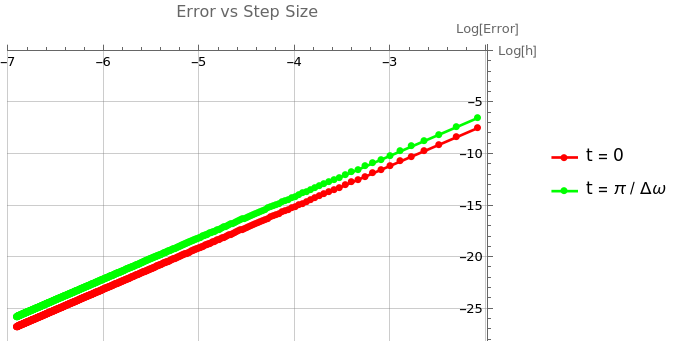
\includegraphics[width=0.75\textwidth]{./../problem4/prob4a.png}
            \caption{}
            \label{fig:graph4a}
        \end{figure}
        As can be seen in the plot, the step size aligns very nicely with the size of the error over many orders of magnitude (as indicated by the logorithm).
\end{enumerate}

\newpage

\begin{ex}
    5 Application in Mode Decomposition
\end{ex}

Create a function to numerically integrate a data-based integrand via two of the following methods:
\begin{enumerate}[label=(\alph*)]
    \item Trapezoid Rule
    \item  2nd order Newton-Cotes
    \item Simpson's \(\frac{3}{8}\) Rule
    \item Euler-Maclaurin Method
    \item  Gauss-Legendre Methods of Orders 2, 4, and 8
    \item Splines
\end{enumerate}

Test the functionality of the integration program on the following functions over the pre-defined intervals:
\begin{align*}
    f_{1} \rb*{ x} & =  e^{x} \cos \rb*{x}, &x \in \sqrb*{0, \frac{\pi}{2}} &\\
    f_{2} \rb*{ x} & =  e^{x}, &x \in \sqrb*{-1, 3} &\\
    f_{3} \rb*{x}& =  
    \begin{cases}
            e^{2x}  & x < 0 \\
            x - 2 \cos \rb*{ x} + 4  & x \geq 0 
        \end{cases}, &x \in \sqrb*{-1,1}
\end{align*}

Plot \(\log(\text{Error} )\) vs \(\log \rb*{h}\) for the three functions using \(n \in \sqrb*{5, 501}\) points.

\begin{sol} 5 \end{sol}

The first part of this exercise involves developing a program to numerically solve an \texttt{integral} struct. The resulting \(\log(\text{Error} )\) should then be compared to the known analytical results with a dependence on the \(\log\) of the stepsize \(h\). The second part of the exercise is to be addressed in a later assignment. 

To solve this task a c program was written and compiled using \texttt{make}. It was then run using \texttt{./integrate.out <function number>} with \texttt{<function number>} one through three.

For the methods of integration it was decided to use the trapezoid rule and Simpson's \(\frac{3}{8}\) rule (SR). The trapezoid rule can be used for any number of points without modification, but the SR required dividing the dataset into sub intervals with 4 points on which SR could be used. It is worth noting that there were in practice \(\frac{\text{numPoints }  - 1}{3}\) sub intervals (rounded down to the nearest whole number). This division into intervals of three is due to the reuse of the last point in an interval as the first point in the next interval. 

Points that did not fit into these subintervals were then integrated by defining a new \texttt{integal} struct and integrating using the trapezoid rule. This resulted in a better approximation than using the only the trapezoid rule, but there was a substatntial loss of accuracy for results that did not fit exactly into the SR subintervals.

The exported data were then plotted using a GNU Plot script.

\begin{figure}[ht]
    \centering
    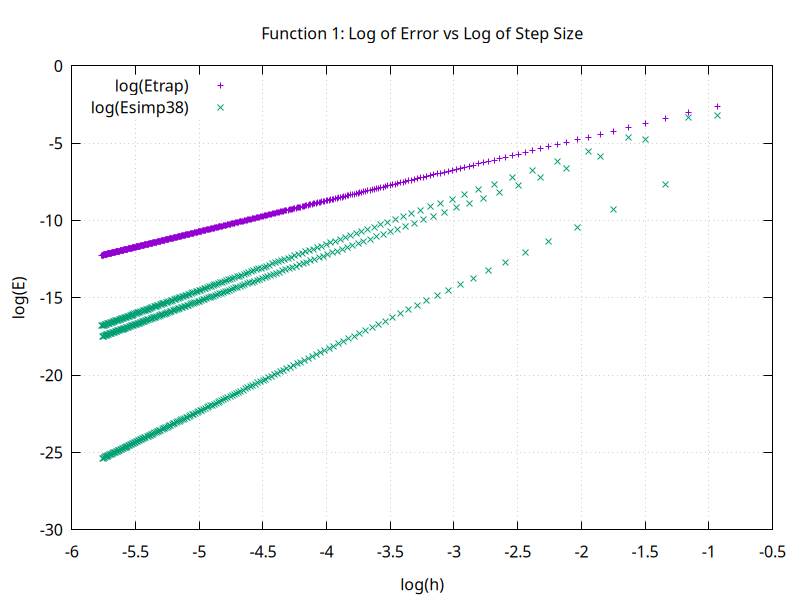
\includegraphics[width=0.75\textwidth]{./../problem5/data/function1.png}
    \caption{Function 1 Plot}
    \label{fig:fnct1}
\end{figure}
\begin{figure}[ht]
    \centering
    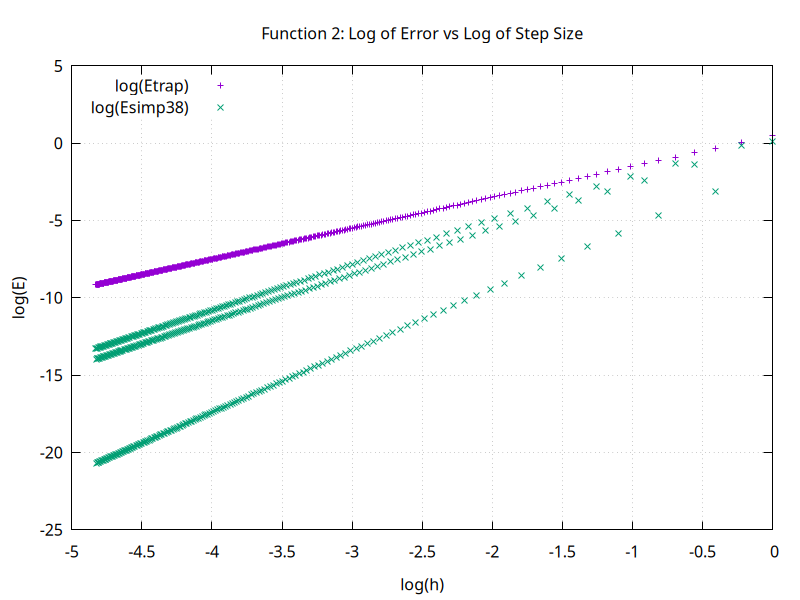
\includegraphics[width=0.75\textwidth]{./../problem5/data/function2.png}
    \caption{Function 2 Plot}
    \label{fig:fnct2}
\end{figure}
\begin{figure}[ht]
    \centering
    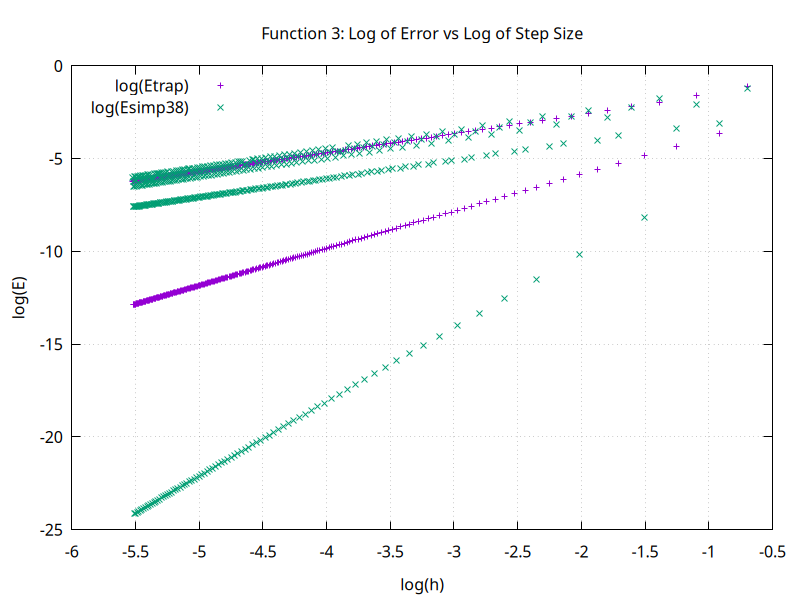
\includegraphics[width=0.75\textwidth]{./../problem5/data/function3.png}
    \caption{Function 3 Plot}
    \label{fig:fnct3}
\end{figure}

As expected, the plots for the SR were usually more accurate, even for the same step size. Results were however inconsistent due to the flucuations in the numbers of steps and the application of the trapezoid rule. 

Though the error of the trapezoid rule seems to consistently decline with smaller step sizes, it is worth noting that it also can flucuate for functions with incontinuities (like function 3).

Higher accuracies could be achieved by using an integration method appropraite to the number of points. Function 1, for example, is well-behaved function that could benefit from numerical integration methods that require more data (like Boole's rule) if the step size is known. The same could be said for function 2. 

Function 3, on the other hand, requires careful consideration of the incontinuity at \(x = 0\), requiring there to be a division into two areas of integration for the highest accuracy possible. 



\end{document}
